\chapter{Open Source}
\label{sec:open_source}

The open source ecosystem%
\marginNote{%
  \marginTitle{Open Source}
    Open source is a philosophical movement that originated as a reaction to the restrictions imposed by proprietary software.
    It encourages collaboration when building software.
    Generally speaking, an open source software will provide the four following freedoms:
    \begin{enumerate}
      \item Freedom to run the program.
      \item Freedom to see the source code.
      \item Freedom to change the source code.
      \item Freedom to distribute the code, modified or not.
    \end{enumerate}
    Generally speaking, open source favors a decentralized software development system.
}
features diverse participants: nerds coding in their basements, and megacorporations with revenues larger than the GDP of entire countries like Google and Facebook.
Reasons for participating to open source projects vary also; from benefiting humanity by developing public goods, to having some fun coding during Sunday evenings, to benefiting from contributions from the community to lower maintenance costs, to making profits with paid services sold on top of open source projects.

Many of the thoughts, models, and ideas proposed here are drawn from a famous essay on management styles in the open source: \citetitle{raymond_cathedral_2001} \cite{raymond_cathedral_2001}.

\section{Business Model}

The vast majority of open source projects do not make money.
This general lack of a business model is an intriguing aspect of this ecosystem.
Many prophesized that it would be the downfall of open source: if you don't make money by contributing, why contribute at all?
In this sense, open source is a public good.
Everyone benefits from the existence of the good, but no one has a personal incentive to make the good exist.
Those that produce the value, i.e.\ the developers, are not the ones that extract it.
This is a case of the tragedy of the commons.
Yet, surprisingly, open source has never been stronger.

Some argue that the lack of monetary incentives is what gives strong quality assurance about the code.
People that contribute to the open source, doing it for free, must care about the software.
And because the quality is better, open source is more successful.
But does caring ensure quality?
And today, billions of dollars depend on open source software, so the reasons to contribute to the open source can be a lot more diverse than only caring about the software.
Some companies pay developers to contribute to open source software they depend on.
And since so much value depends on open source software, some contributors are also adversarial agents, trying to perform supply chain attacks to steal some of that value.

We do not know of a good explanation for the open source miracle.
Why does it strive when there is no business incentive?
Maybe, the fundamental semantics of computer sciences have something to do with it.
In the digital realm, creating copies is almost free.
Therefore, it is enough that a single individual decides to create open source software for everyone to benefit, and through the great diversity in humankind, there are enough people ready to contribute for reasons personal to themselves.

Yet open source faces new challenges today, like supply chain attacks.
Open source software comes with no guarantees: you do not have to pay to use them, but there will be no one either to help you when your business is out, because of a technical issue in the open source library you use.
The quality of the documentation and the tests are up to the developers.
There are no contracts to provide financial counterparties in the event of failure, no one that you can sue.
One uses open source at its own risk.

A recent, yet highly damaging, example of this issue is the security issue in the logging library called \texttt{log4j}.
Logging, especially in corporate software running 24/7, is an important feature, as it gives insight into what is happening inside the program.
This, in turn, enables debugging, tracing and gives visibility in real time over the potential problems a program might be experiencing.
It is the voice of a program.
And when \texttt{log4j} was released, it introduce a plethora of concepts and features that did not exist at the time, yet were highly valuable (like logging to a distant server, rotating logging files, logs formatting, outputting to various sinks, etc.).
So the library was soon used by many Java programs, especially corporate programs.
Time passed by, and new libraries were created on top of \texttt{log4j} so that developers were often using \texttt{log4j} without even knowing it.
Yet, at the core of the library was a security issue that enabled running arbitrary code on the machine running the program, i.e.\ a security breach of the worst, most dramatic kind.
On December 9\textsuperscript{th}, 2021, the breach was discovered.
To give an idea of the problem, the director of the \textsc{cisa}%
\marginNote{%
  \marginTitle{\textsc{cisa}}
  The Cybersecurity and Infrastructure Security Agency is the American body responsible for analyzing cybersecurity threats in the United States of America.
} described the flaw as the \enquote{most serious} she had seen in her career \cite{noauthor_cisa_nodate}, and Google analyzed soon after that it impacted around 8\% of all the packages on the most popular Java package repository, Maven \cite{noauthor_understanding_nodate}.
Those packages are used by millions of servers throughout the Internet.
Among some of the most widely known services that could be exploited: Cloudflare, iCloud, Minecraft, Steam, Tencent, and Twitter.
The exploit received the highest CVSS severity rating of 10.
The breach is particularly easy to exploit, but patching the vulnerability is complex, also because changing existing features might break some software using them.
And the \texttt{log4j} library was maintained by a single individual, \texttt{rgoers}, that had three sponsors on GitHub.

\begin{figure*}[ht!]
  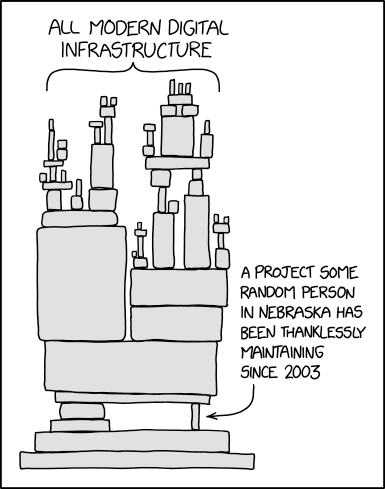
\includegraphics[width=0.5\linewidth-0.5\columnsep]{images/dependency.png}\hspace*{\columnsep}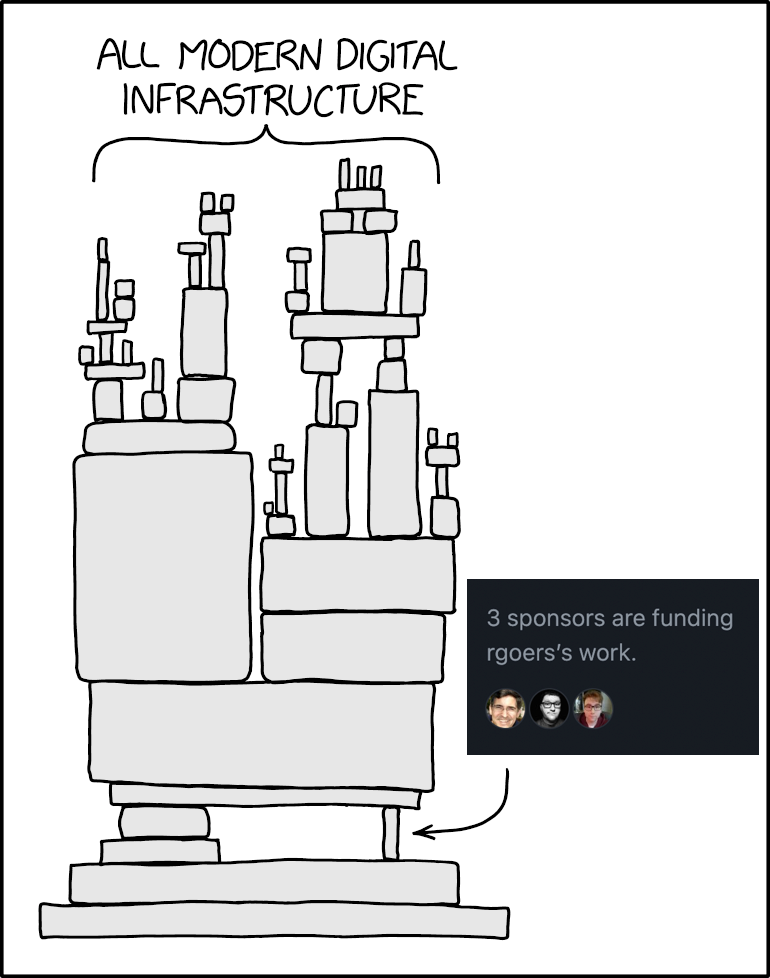
\includegraphics[width=0.5\linewidth-0.5\columnsep]{images/sponsors.png}
  \caption{\label{fig:log4j_dependency}A well-known \texttt{xkcd} meme about modern days software, and a variation of it created specifically for the \texttt{log4j} security breach.}
\end{figure*}

In such circumstances, it is not so surprising that quality assurances are not a top priority for the maintainer of the code.
Filippo Valsorda, a member of the \texttt{golang} team at Google, wrote on this topic that \textcquote{filippo_valsorda_professional_2021}{the role of open source maintainer has failed to mature from a hobby into a proper profession. The catastrophic consequences are almost a daily occurrence. [...] [T]he status quo is unsustainable.}

Maybe open source does not need a business model to survive, live on and thrive, but the world needs open source to have one.

\section{Key Aspects of Open Source}

\subsection{Stakeholders}

In any open source project, there are multiple stakeholders.
The two stakeholders which are always present are:

\begin{description}
  \item[Developers]
  	They create, improve and maintain the project.
  \item[Users]
  	They draw some value from the project.
  	Users can be other developers that use the current project as part of their project, e.g.\ in the case of a software library; or users can be nontechnical people like users of an open source app on a phone.
\end{description}

There is a fundamental imbalance in the open source ecosystem, which is that it is often much easier to get some feedback from developers that know the platforms used to collaborate on code (like GitHub) than it is to get feedback from users.
When users are developers, this is not such a big issue.
But when users are nontechnical, getting some feedback to prioritize the most valuable features can be harder.
Corporate products will often measure in some capacity user behaviors.
This is done much more seldomly in the open source world, first, because it requires a server to receive and store those data for which someone needs to pay (but the projects generally do not make any money), and second because tracking users goes against the open source narrative.
Finding ways to get feedback from the users might make the open source provide more value to humanity.

\subsection{Scales of Open Source Projects}

Open source can operate at various scales.
Many projects have one developer and few users.
Some others attract hundreds of developers and have millions of users like the Python library \texttt{pandas}.

Hereafter we outline three developer community scales that are useful to keep in mind when developing management systems for open source.
Whatever the system, it should adapt well to all three, or it should be specified to which category it applies.

\begin{description}
  \item[Small]
    One to three developers, strong vision, tight coordination, and intentional core design.
    No need for explicit management; it will most probably happen in an organic way, or through the original leader of the project.
  \item[Medium]
    Four to fifteen people, traditional management might bring more benefits than drawbacks at this scale, e.g.\ avoiding duplication of effort, making sure no detail is forgotten, etc.
  \item[Large]
    Management becomes unmanageable.
    Better to embrace anarchy at this point.
\end{description}

\subsection{Core and Halo Developers}

Open source relies strongly on its developer community to make progress.
Yet, not all developers contributing to the project are equal.
Some are more involved, others are less.
As proposed in \citetitle{raymond_cathedral_2001}, developers can generally be divided into two categories:

\begin{description}
  \item[Core]
  	Those are the developers which are highly involved in the project.
  	They generally know the codebase well and contribute regularly.
  	Being at the center of the project, they often coordinate the project in some way.
  \item[Halo]
  	Halo developers are those that contribute a couple of times, maybe only once.
  	They have a specific feature that they want to be implemented or a bug that they want to be fixed.
  	However, they generally don't know the codebase well and it might be hard for them to know where the feature that they want to build needs to go.
  	Having some guidelines for contributors to help them find their way is often useful.
\end{description}

\subsection{Management Styles}

There are probably as many management styles for open source as there are open source projects.
However, the book called \citetitle{raymond_cathedral_2001} \cite{raymond_cathedral_2001}, a famous essay on this topic, describes the models used by two different projects and uses them as general categories:

\begin{description}
  \item[Cathedral]
    Centralized, one or few leaders that coordinate the work of many subordinates, also called \textit{top-down}.
    Coordination happens \textit{a priori}.
    Access to the project's development might be restricted to only trusted developers.
    The leaders provide/impose their vision for the project.
    Code is released once a coherent set of tested features have been added, which generally happens at fixed deadlines.
    A famous program developed using this framework is GCC, the GNU C Compiler.
  \item[Bazaar]
    No management of who should do what.
    Everyone can contribute, the development process is completely public and somewhat anarchistic, also called \textit{bottom-up}.
    Coordination happens \textit{a posteriori}.
    Code is released continuously, at no set deadlines.
    This model was spearheaded by Linus Torvald, and is still used to develop the Linux kernel.
    This model is probably the most cited reason for the kernel's success.
\end{description}

For the bazaar development style to work efficiently, a large enough base of developers needs to be involved.
\citeauthor{raymond_cathedral_2001} proposes, to bootstrap a bazaar-managed project, that developers be attracted by providing a vision and some working prototype.
Providing a clear vision ensures that only align people take part in the project, in the beginning at least.
Having less aligned people later is much less of an issue that having unaligned people in the beginning, as it causes a lot of disruption.
Further, building a working prototype, even if very poor, gives something tangible that people can play with.
It gives some insight into what the finished product might look like, which helps bring people on board.
The book further postulates that a flat organization with only a few project maintainers for the project's coherence is the better way forward.
The power of a large decentralized community beats a single mind, however brilliant it is.

Note that \citetitle{raymond_cathedral_2001} was written in 1997.
Git was released in 2005, so the book describes a time when mailing lists were used commonly for coordination of software developers and \emph{git did not exist}.

\subsection{\textsc{Snafu} Principle}

Some further argument in favor of having as little hierarchy as possible is named the \textsc{snafu} principle:
\blockcquote{noauthor_snafu_nodate}{True communication is possible only between equals because inferiors are more consistently rewarded for telling their superiors pleasant lies than for telling the truth.}

\textsc{Snafu} predicts a progressive disconnection of decision-makers from reality, which is an argument regularly used by hackers and proponents of flat hierarchies why strongly hierarchical systems often fail.
A fable illustrating the \textsc{snafu} principle is included in \cref{sec:snafu_fable}.

\section{GitHub's Influence on Open Source}

A major actor in the open source ecosystem today is GitHub \cite{noauthor_github_2022}.
The platform was created in 2008 and provides free, centralized hosting of git remotes, plus many social coding features.
The company was acquired in 2018 by Microsoft for \$7.5 billion.

The original vision behind \texttt{git} was not to use walled, single, centralized remotes as we do today.
The initial vision was actually extremely flexible; \texttt{git} should be able to fit any workflow.
This makes using \texttt{git} difficult for newcomers because \texttt{git} can be used in so many different ways.
Of course, humans like simplicity, and so we deeply associated using \texttt{git} with using some socially-enabled remote because it was simpler; so much, so that many people now confuse \texttt{git} and GitHub.
But the design of \texttt{git} makes it possible to collaborate on code using decentralized workflows.
Only, as those workflows are generally more complex both technically and for the mind, they are not widespread.
There are also no mature technical solutions to working in a decentralized fashion on code as of August 2022.
But some projects are trying to implement a decentralized way to collaborate on code using \texttt{git}, like Radicle (see \cref{sec:radicle} for more details).

GitHub's offering was a game changer, it changed the face of open source.
The interface enabled people to build faster, provided new features like \textsc{ci/cd}%
\marginNote{%
  \marginTitle{\textsc{ci/cd}}
  Continuous Integration/Continuous Deployment is an umbrella term that designates many things, but it generally boils down to having some scripts automatically executed every time a commit is made on a git branch, or every time a merge request is initiated.
  This idea is powerful because it enables developers to automate many boring tasks, like executing tests before merging which increases the assurances on code quality a lot.
  This idea can be pushed further, for example, it is possible to package and deploy your code whenever you commit to the release branch.
  In the world of microservices and web-based products, this means that developers can stop worrying about putting their code online: the code hosting platform will automatically execute a script that will do it for them.
}, merge requests%
\marginNote{%
  \marginTitle{Merge Request}
  A \textit{merge request} is a process to submit code for merging on a protected branch.
  The process can include or mandate code proofreading, successful execution of \textsc{ci/cd} pipelines, including tests, and acceptance by a quorum of permissioned members.
  It often also features a discussion thread which enables people to comment on and discuss about the code.
}, issues%
\marginNote{%
  \marginTitle{Issues}
  Issues are threads that people can use to ask for new features or to report bugs.
  It enables getting some feedback from the community and the users, although nontechnical users probably do not use this channel as it often requires a technical background to be used (an account on GitHub, adding some trace of the bug, tagging correctly, abiding by the contributing guidelines, etc.).
}, comments, stars%
\marginNote{%
  \marginTitle{Stars}
  Developers can give a \emph{star} to the repositories that they like.
  This feature created a reputation system for open source repository: many stars indicate a software used and liked by many.
  Having few stars means that the community behind a project is smaller, hence the code might not receive enough attention to provide strong quality assurances.
}, sponsors%
\marginNote{%
  \marginTitle{GitHub Sponsor}
  GitHub Sponsor is a program created by GitHub whose goal is to provide funding to the open source ecosystem.
  Projects can register on the program, then a \enquote{Sponsors} button will appear on the project's page, enabling people to make one-time or recurring donations to the project.
  While the intention is good, the effects of the functionality have so far been negligible.
}, and so it has become the largest database of open source code in the world with more than 40 million public repositories listed.
Because GitHub is used so much, the functionalities provided by GitHub shaped the history of open source development.
People now regularly conflate \texttt{git} and GitHub, are not so sure which of the two provides what functionalities; this is the extent to which GitHub has become the \textit{de facto} standard.

Among the features offered by GitHub is a permission system.
When a repository is created, its initiator originally has every right on it, and others have none.
Afterward, the repository owner can grant various additional rights to GitHub accounts.
Some of the permissions include: pushing to the repository (can be set per branch) and merging branches (can be set per branch too).
This is a centralized approach to permissions, similar to what is used in the corporate world, but it goes somewhat against the narratives associated with open source, like anarchy and decentralization.
More democratic management systems, like voting systems, were never offered by GitHub, and so the recent history of open source never featured decentralized, permissionless, or trustless governance systems.

\section{Trustlessness Open Source}

Why do we care about governance of open source projects being or becoming decentralized?
Because it enables users of the project to trust the project as a whole, even if some members mean harm to the project or its users.
It makes open source trustless, by improving the following properties:

\begin{description}
  \item[Security]
  	More people involved also implies that it will be more difficult to include some adversarial code in the project.
  	One would need to circumvent code reviews so that no one discovers the adversarial code in the codebase in the future.
  \item[Longevity]
		Having more active contributors gives stronger guarantees that the project will live on because it increases the probability that someone will maintain the project in the future.
    If we consider the Linux project, which is highly centralized around Linus Torvald, one might ask what will happen if Linus dies suddenly in a car accident.
    It is possible that the community behind the project finds a new governance process rapidly and the project only suffers a minimal impact.
    But it can also be that the community explodes and we end up with multiple subcommunities, each maintaining their fork of the Linux kernel.
    Are you willing to take such a risk?
    A decentralized approach features better properties in our opinion.
  \item[Faster Progress]
    People are generally more involved in a project if they have a say in it.
		More people involved means more features built, more bugs discovered, more bug fixes, etc.
\end{description}

